\chapter{Expunerea tehnologiei}

\subsection{Serviciul NLU}
\begin{figure}[h]
	%\centering
	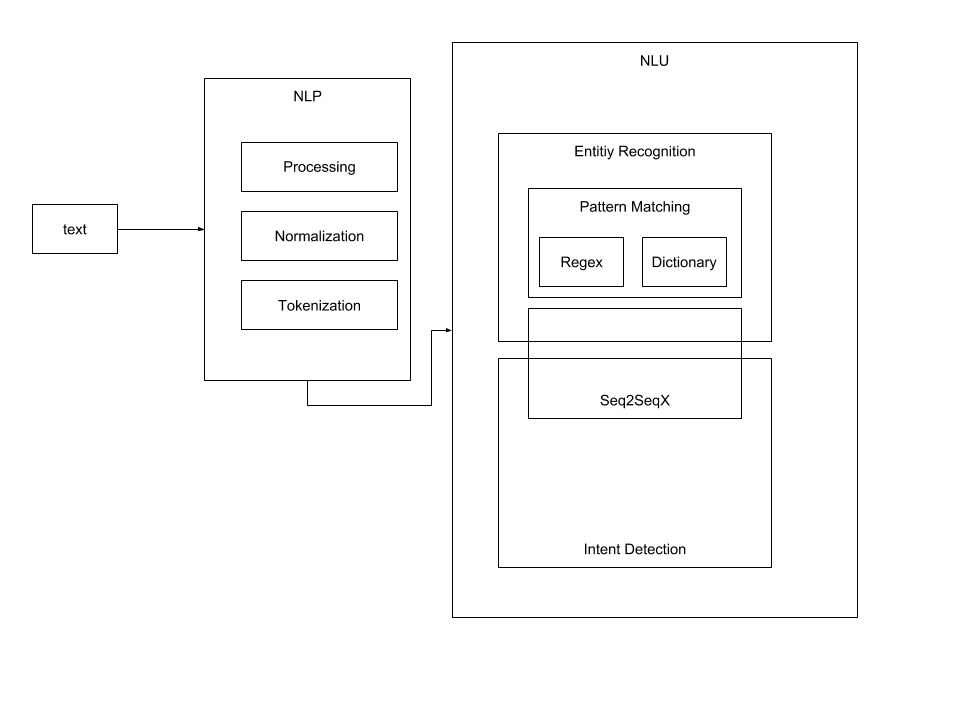
\includegraphics[scale=0.5]{nlu_architecture.png}
	\caption{Arhitectura serviciului de NLU}
	\label{fig:nlu_arch}
\end{figure}

\section{Tehnologii folosite}

Desemnarea tehnologiilor open source folosite ca dependințe poate fi văzută la prima vedere o alegere ușoară, însă este nevoie de o analiză mult mai amănunțită în ceea ce privește specificul proiectului.
Pentru această lucrare am luat în considerare următorii factori: complexitatea de a descrie o rețea neuronală să fie cat mai simpla, dar să reflecte cat mai bine tot procesul matematic din spate, flexibilitatea de a putea jongla cu diferite arhitecturi de rețele. Evident viteza și eficiența cu care aceste biblioteci rulează, dar și dispozitivele pe care ele rulează (CPU/GPU).

\subsection{Python}

Python a fost creat la începutul anilor 1990 de Guido van Rossum la Stichting Mathematisch Centrum (CWI) în Olanda ca un succesor al limbajului, ABC. \cite{pythonhistory}

Python este un limbaj de programare puternic și ușor de învățat. El are structuri de date implementate la un nivel înalt și reprezintă o abordare simplă, dar eficientă a programării orientate pe obiecte. Python are o sintaxa elegantă, ce impune o dactilografiere dinamică, împreună cu natura sa de limbaj interpretat, reprezintă un instrument ideal pentru scripting și dezvoltarea rapidă a aplicațiilor în multe domenii, pe majoritatea platformelor.

Interpretorul Python și biblioteca standard extinsă sunt disponibile gratuit în format sursă sau binar pentru toate platformele majore pe site-ul Web Python. În același site sunt conținute, de asemenea, distribuții și indicii pentru mai multe module, programe, instrumente și documentație suplimentară.

Interpretorul Python este ușor de extins cu noi funcții și tipuri de date implementate în C sau C++ (sau alte limbaje apelabile din C). Python este de asemenea potrivit ca o extensie pentru aplicații personalizate.
\cite{python_tutorial}

\subsection{Numpy}

Numpy este un acronim pentru "Numeric Python" sau "Numerical Python". El este un pachet fundamental pentru calculul științific in Python, ce furnizează funcții precompilate care se execută rapid cu scopul de a efectua operațiile matematice de rutină.  Mai mult decât atât, NumPy îmbogățește limbajul de programare cu structuri puternice de date pentru calculul eficient de vectori si matrice, implementarea sa suportând chiar și dimensiuni uriașe.

SciPy (Scientific Python) este adesea menționat atunci când vine vorba de NumPy. SciPy extinde capabilitățile NumPy cu alte funcții utile pentru minimizare, regresie, transformate Fourier și multe altele.

Atât NumPy și SciPy nu sunt de obicei instalate în mod implicit. NumPy trebuie să fie instalat înainte de a instala SciPy. 

NumPy se bazează pe două module anterioare Python care se ocupă cu matrice. Unul dintre acestea este Numeric. Numeric este ca NumPy un modul Python pentru înaltă performanță de calcul numeric, dar este învechit în zilele noastre. Un alt predecesor al NumPy este Numarray, care este o rescriere completă a modulului Numeric, dar este învechit de asemenea. NumPy este o fuziune a celor două, adică este construit pe codul lui Numeric dar cu caracteristicile lui Numarray.

\subsection{PyTorch}

% todo de citat sursa din https://pytorch.org/tutorials/beginner/blitz/autograd_tutorial.html

PyTorch este o bibliotecă software ce oferă un cadru de lucru cu algoritmi de invățare automată. Se prezintă ca o variantă de Numpy care poate rula pe placa video, având tot odată și capacitatea de autodiferențiere atunci când este nevoie să antrenăm, spre exemplu folosind metoda gradientului descendent.

\textbf{Diferențiere Automată}

Componenta cheie a rețelelor neuronale din PyTorch este pachetul \textit{autograd}. El oferă diferențierea automată pentru toate operațiile cu \textit{tensori}. Este un cadru de definire a operațiilor (forward dar și backward) la momentul execuției, ceea ce înseamnă că pasul de backpropagation este definit de modul în care este rulat codul.

\textbf{Tensor}

\textit{torch.Tensor} este clasa centrală a pachetului. Dacă se setează atributul \texttt{.requires\_grad} ca  \texttt{True}, se va începe urmărirea tuturor operațiilor în care acesta intervine. După ce se termină calculul, se poate apela \texttt{ backward()} pentru a calcula automat toate derivatele, iar gradientul pentru acest tensor va fi acumulat în atributul \texttt{.grad}.

Pentru a opri tensorul din istoricul de urmărire, se apelează \texttt{.detach()} care detașează tensorul de istoricul de calcul și care împiedica urmărirea viitoarelor calcule.

Mai există încă o clasă care este foarte importantă pentru implementarea autodiferențierii - și anume \textit{Function}.

Tensorul și funcția sunt interconectate și construiesc un graf aciclic, care codifică un istoric complet al calculelor. Fiecare tensor are un atribut  \texttt{.grad\_fn} care se referă la o funcție care a creat tensorul (cu excepția tensorurilor creați de utilizator unde - \texttt{.grad\_fn = None}).